\label{ch4}
\section{簡介}
在第\ref{ch3}章中,嘗試了直接將語音文件跟語音查詢詞編碼成向量,進行口述詞彙偵測。雖然表現不如非監督式的動態時間規劃,但至少實作出可以捨棄語音辨識系統的口述詞彙偵測。第\ref{ch3}章中,直接將語音查詢詞變成一個向量是很合理的,因為語音查詢詞只包含完整的查詢詞,並無多餘的部分,但語音文件為一整個段落,包含了許多並非查詢詞的資訊,導致產生出來的語音文件向量喪失了查詢詞的特徵。即使後面分類器的複雜度在高,但因語音文件向量中喪失了查詢詞特徵,所以無法準確的分辨。本章將專注式機制引入,專注式機制可以使模型專注在某個地方,將多餘的資訊濾除。藉由專注式機制使模型能夠關注在查詢詞的部分,可以有效保留著查詢詞特徵在產生出來的語音文件向量中,則不會分心在其他非查詢詞的部分。所以本章藉由專注式機制產生出較好的語音文件向量,可以保留著查詢詞的部分,不會被其他多餘的詞彙影響,以提升口述詞彙偵測的效能。
\section{專注式機制}
專注式機制,在近年漸漸受到大家重視,專注式機制最早被應用於機器翻譯的領域上,該系統為先前\ref{seq2seq}章提到的編碼器-解碼器遞迴神經網路,能提供端對端機器翻譯。而該系統的特點為能夠根據前一個時刻的輸出,去側重當今時刻的資料中重要的部分;如此這種根據狀況進行「挑選」的技能是先前的其他類神經網路所無法比擬的。
現已出現一些模擬專注力的神經網絡架構,如記憶網絡(Memory
Network)~\cite{sukhbaatar2015end}、類神經圖靈機(Neural Turing
Machine)~\cite{graves2014neural}、 動態記憶網路(Dynamic
Memory
Network)~\cite{kumar2015ask}等等,這類模型統稱專注式模型(Attention-based
Model)。

專注式模型常應用在問答(Question
Answering,QA)系統上,讓機器可以針對提出的問題,回答正確的答案。當使用者輸入問題時,專注式模型可以幫助機器從資料庫中選擇相關資料,而將專注力放在相關的資料上,避免其他無關資訊干擾,藉此得到問題的答案。問答系統甚至已經從文字擴展到多媒體,機器可以依據圖片回答相關問題(如:圖中的人穿什麼顏色的衣服)~\cite{agrawal2015vqa},而專注式機制可以幫助模型將重心放在圖片中人的衣服上,來判斷衣服的顏色,不會受到圖片中其他物件影響。不只如此,專注式模型也被應用在自動新聞摘要~\cite{rush2015neural}、自動產生圖片/影像說明~\cite{xu2015show}、語音辨識~\cite{chan2016listen}~與機器自動翻譯等任務上~\cite{bahdanau2014neural}。

受到這些啟發,將專注式機制應用於口述詞彙偵測。在第\ref{ch3}章中,編碼器最主要的難處是當輸入序列相當長時,可能會有比較多雜訊在其中、或者許多部分是與整體資訊無關的,這些或多或少都會影響編碼出來的語音文件向量,進而影響分類器判斷結果的正確率。因此我們希望透過專注式機制的特性,建立在原本長短期記憶神經網路就能處理序列問題的基礎上,再自動從序列中挑出重要的部分並且忽略其餘跟查詢詞無關的部分,使其語音文件向量能夠包含著查詢詞的資訊,使平均準確率能夠提升。
\section{模型架構}
\subsection{系統架構簡介}
\begin{figure}[h]
\centering
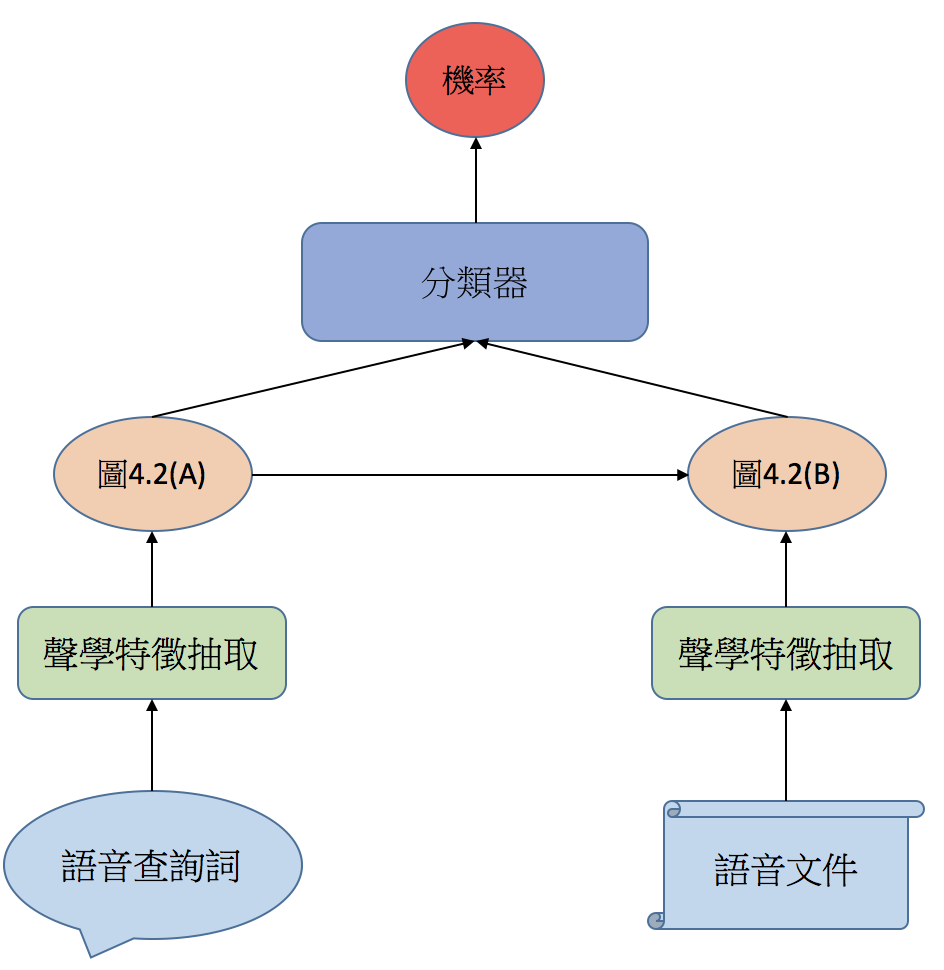
\includegraphics[scale=0.5]{images/ch4_model.png} 
\caption{模型架構圖}
\label{ch4_system}
\end{figure}
圖\ref{ch4_system}為本章節之系統架構圖。系統輸入部分包含了語音查詢詞跟語音文件,分別會經由聲學特徵抽取,轉變為39維的梅爾倒頻譜係數。首先,語音查詢詞的聲學特徵序列如同第\ref{ch3}章一樣被壓縮編碼並表示成為一向量,此向量稱之
$V_Q$ ,此部分會在\ref{ch4_query_vec}章在做介紹。產生出了 $V_Q$
,於\ref{ch4_doc_vec}章中將使用專注式機制找出跟語音查詢詞有關的部分,產生出較好的語音文件向量
$V_S$ 。最後,將 $V_Q$ 跟 $V_S$ 藉由分類器去預測查詢詞出現在文件中的機率,將在\ref{ch4_classify}章中作介紹。
\subsection{語音查詢詞之向量表示法}
\begin{figure}[h]
\centering
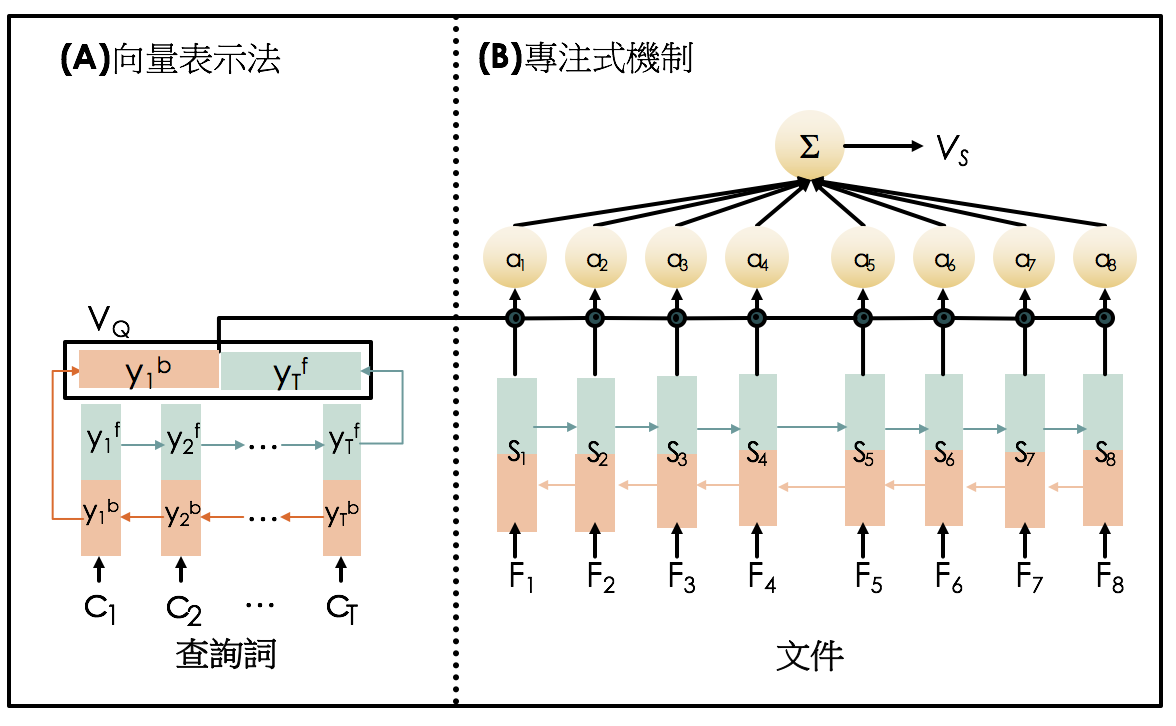
\includegraphics[scale=0.7]{images/ch4_att.png} 
\caption{專注式機制流程圖}
\label{ch4_att}
\end{figure}
\label{ch4_query_vec}
圖\ref{ch4_att}(A)為抽取 $V_Q$ 向量的介紹,將一連串的聲學特徵序列轉換為
$V_Q$ 的過程。輸入的查詢詞為
一長度T的序列,$C_1$, $C_2$,
...,$C_T$,其中 $C_i$ 均為39維梅爾倒頻譜係數。使用雙向式長短期記憶網路(Bidirectional
Long Short-term Memory
Network)作為編碼器的模型;其在輸入語音序列時,一個時間點只會讀取一個音框進去。在圖\ref{ch4_att}(A)中的第t個時間點時,正向(forward)長短期記憶網路的隱藏層輸出表示為
$y_t^f$ 、而反向(backward)長短期記憶網路之隱藏層輸出表示為 $y_{t}^b$
。在讀入所有的輸入序列之後,可在正向長短期記憶網路的最後一個時間點獲得一組隱藏層輸出向量
$y_{T}^f$ 、在反向長短期記憶網路的第一個時間點獲得 $y_{1}^b$
,並把他們串聯起來作為查詢詞的向量表示法 $V_Q$ , $V_Q
= [y_T^b || y_1^f]$ 。
\subsection{專注式機制與語音文件表示法}
在圖\ref{ch4_att}(A)中獲得查詢詞的向量表示法 $V_Q$
之後,之後將利用畫重點機制配合遞迴神經網路來對於語音文件的序列進行編碼,得到向量
$V_S$
,如圖\ref{ch4_att}(B)所示,語音文件的內容其實是一相當長的聲學特徵序列,但圖中我們簡化為八個音框,我們同樣使用雙向式長短期記憶網路來作為編碼的工具,其中在第t個時間點時,輸入詞彙的向量表示
$S_t$ 為正向長短期記憶網路與反向長短期記憶網路隱藏層輸出的串聯,$S_t
= [ y_t^f || y_t^b ]$。
接著我們引入專注式機制,來衡量查詢詞向量 $V_Q$
與語音文件內音框的關聯性高低,第 t 個時間點的語音文件向量 $S_t$
之專注式權重 $\alpha_t$ 為 $V_Q$ 與 $S_t$ 的相關程度,$\alpha_t=
S_t \odot
V_Q$,其中$\odot$表示兩向量之間的相關程度運算。相關程度的運算自己定義的,可以是簡單的歐式距離(Euclidean
Distance)、餘弦相似性(Cosine Similarity),也可使用類神經網路來計算,將兩向量丟入類神經網路去計算相關程度。
在本章中採用餘弦相似性當作相關程度,如式子\ref{cos_sim}所示:
\begin{equation}
	\label{cos_sim}
	\alpha_t = S_t \odot V_Q = \frac{S_t \cdot V_Q}{|S_t||V_Q|}
\end{equation}

接下來,對於所有的專注式權重 $\alpha_t$ 進行正規化,成為
$\hat{\alpha}_t$ ,正規化的方式有兩種。
\begin{itemize}
	\item{尖銳(Sharpening)正規化}
		
		我們將專注式權重透過軟式最大化(Softmax)之活化函數進行正規化:
		\begin{equation}
			\hat{\alpha}_t =
			\frac{exp(\alpha_t)}{\sum_{t=1}^{T} exp(\alpha_t)}
		\end{equation}
		由於可以確實降低資料的雜訊,此方式已被現存其餘專注式機制的相關研究所廣泛使用。
	\item{平滑(Smoothing)正規化}
		
		尖銳正規化偏好於注意一個點,因此一整個專注式權重集 $
		\boldsymbol{\alpha}
		= (\alpha_1,\alpha_2, ...,
		\alpha_T)$
		可能只會有某個向量 $\alpha_t$ 的權重特別高,其餘資訊皆被捨去。這樣的特性有可能降低口述詞彙偵測的表現。因此另外設計了一種正規化表示法,能夠考慮更多重要的點,此種方式也讓模型的多樣性因而增加。我們將原本算式中的指數函數改成S型函數(Sigmoid Function)$\sigma$:
		\begin{equation}
			\hat{\alpha}_t =
			\frac{\sigma(\alpha_t)}{\sum_{t=1}^{T}\sigma(\alpha_t)}
		\end{equation}

\end{itemize}

最後對於所有的語音文件向量 $S_t$
進行加權平均,使用的權重便為正規化後的專注式權重 $\hat{\alpha_t}$
,得到代表語音文件的向量 $V_S$,$V_S
= \sum_{t} \hat{\alpha_t} S_t$。
\label{ch4_doc_vec}
\subsection{分類器}
最後模型的輸出分數由分類器來決定的。分類器有很多種模型,常見的有支撐向量機(Support
Vector Machine)、類神經網路、貝氏分類器(Bayes
classifier)、決策樹(Decision
Tree)等等。在此章中,以多層類神經網路當作分類器,另外還使用語音文件向量 $V_S$
跟語音查詢詞向量 $V_Q$ 的餘弦相似度當作輸出分數為兩種產生分數的方式。
\label{ch4_classify}
\section{實驗與分析}
\subsection{基準實驗與實驗設定}
實驗語料仍使用LIBRISPEECH的英文語料,從train-clean-360取出70,000筆查詢詞跟語音文件配對,查詢詞共500個。測試語料分成測試集1(查詢詞聲學特徵跟訓練集相同)、測試集2(查詢詞聲學特徵跟訓練集不同)、測試集3(查詢詞未出現在訓練集)。
測試集$1$跟測試集$2$,皆約30個查詢詞,共1,500筆的測試查詢詞跟語音文件配對。測試集$3$,約100個查詢詞,共10,000筆測試查詢詞跟語音文件配對。

基準實驗為片段式動態時間校準,在測試集$1$得到平均準確率0.6173,測試集$2$得到平均準確率0.5778,測試集$3$得到平均準確率0.5678。

損失函數仍為交叉熵式\ref{eq:ch4_LCE}
\begin{equation}
\label{eq:ch4_LCE}
L_{CE}(\bold{x}, \bold{y} , \theta) = KL(\bold{y} || f_{\theta}(\bold{x}))= KL( \bold{y} ||\hat{\bold {y}} )  = - \log \hat{y}_{l} 
\end{equation}
其中KL為克雷散度,$\bold{y}$為正確答案,$\hat{\bold{y}}$為模型預測之結果,$\hat{y_l}$為模型給正確標籤的分數。最佳化演算法採用Adam演算法~\cite{kingma2014adam},一種改良SGD演算法。採用二次正規化並給予權重$0.001$,來限制模型避免過度貼合。
\subsection{實驗結果與比較}
\begin{table}[ht]
	 \centering
	 \caption{專注式遞迴類神經網路實驗結果}
	 \label{table:ch4_att_exp}
	 \begin{tabular}{|c|c|c|c|c|}
		 \hline
		 \multicolumn{2}{|c|}{模型架構} & 測試集1 & 測試集2 & 測試集3 \\
		 \hline
		 \multicolumn{2}{|c|}{基準實驗} & 0.6173 & 0.5778 & 0.5678\\
		 \hline
		 \hline 
		 編碼器模型 & 分類器模型 & 測試集1 &測試集2 & 測試集3 \\
		 \hline
		 \multirow{3}{*}{長短期記憶網路} & 類神經網路 &
		 {\color{red}0.6523} &0.6246 & 0.5754\\
		 \cline{2-5}
		 & 餘弦相似度& 0.6331 & 0.6043 & 0.5746 \\
		 \cline{2-5}
		 & 結合模型 & 0.6268 & 0.6370 & 0.5759 \\ 
		 \hline
		 \multirow{3}{*}{雙向長短期記憶網路} & 類神經網路 &
		 0.6355 & 0.6187 & 0.5664\\
		 \cline{2-5}
		 & 餘弦相似度& 0.6254 & 0.6144&0.5663\\
		 \cline{2-5}
		 & 結合模型 &0.6192&0.6244&0.5793 \\
		 \hline
	   \end{tabular}
\end{table}


表\ref{table:ch4_att_exp}上的類神經網路架構為$128-64-32-2$,結合模型為將查詢詞向量跟語音文件向量的餘弦相似度也當作類神經網路的輸入,也就是類神經網路的輸出為查詢詞向量、語音文件向量及兩向量之間的餘弦相似度。

從表中可以看出雙向長短期類神經網路的表現都不如單向長短期類神經網路,因雙向成短期類神經網路的模型較複雜且參數較多,產生出明顯的過度貼合的問題,使測試集的表現都比較差。再者,雙向模型在語音辨識跟問答系統都有顯著的進步,但是現在的目標可以類似語音訊號配對,並不是要領解文意或是辨識文字,雙向的模型則可能無法有顯著的進步。

專注式機制確實幫助了模型在測試集$1$跟測試集$2$中打敗基準實驗,不論分類器為類神經網路和簡單的餘弦相似度都表現不錯。從表中可以看出類神經網路的強大推廣性,在語者改變的情況,類神經網路還是能夠判斷出語音查詢詞出現與否,也證明了模型並非只是單純記憶語音訊號而是從中學習出語音查詢詞的聲學組型(Acoustic
Pattern),而簡單的餘弦相似度的表現就有落差,無法與類神經網路有著相同的推廣性。但所有模型在未看過之查詢詞(測試集$3$)表現就表現一落千丈,無法學習出未出現在訓練語料之查詢詞的聲學組型。

\subsection{結合基準實驗}
\begin{table}[ht]
	 \centering
	 \caption{結合基準實驗之結果}
	 \label{table:ch3_late_fusion}
	 \begin{tabular}{|c|c|c|c|c|}
		 \hline
		 \multicolumn{2}{|c|}{模型架構} & 測試集1 & 測試集2 & 測試集3 \\
		 \hline
		 \multicolumn{2}{|c|}{基準實驗} & 0.6173 & 0.5778 & 0.5678\\
		 \hline
		 \hline 
		 編碼器模型 & 分類器模型 & 測試集1 &測試集2 & 測試集3 \\
		 \hline
		 \multirow{3}{*}{長短期記憶網路} & 類神經網路 &
		 0.6523 &0.6246 & 0.5754 \\
		 \cline{2-5}
		 & 餘弦相似度& 0.6331 & 0.6043 & 0.5746 \\
		 \cline{2-5}
		 & 結合模型 & 0.6268 & 0.6370 & 0.5759 \\ 
		 \hline
		 \hline
		 \multicolumn{2}{|c|}{與基準實驗結合後} & 測試集1 &測試集2
		 &測試集3 \\
		 \hline
		 \multirow{3}{*}{長短期記憶網路} & 類神經網路 &
		 {\color{red}0.6720} & 0.6340 & 0.5868\\
		 \cline{2-5}
		 & 餘弦相似度& 0.6433&0.6002&0.5843 \\
		 \cline{2-5}
		 & 結合模型 &0.6451&0.6309	&0.5808 \\
		 \hline
	   \end{tabular}
\end{table}

這一小節中,將基準實驗的分數跟模型預測的分數做結合,希望能夠藉由結合兩者的模型,使其平均準確率在更加進步。從表中可以看出,當模型表現跟基準實驗表現都不錯時,兩者的分數有互補的效果,如測試集$1$所表現的情況。然而若其中某個模型表現較差,則結合之後的結果,都略微退步,如測試集$2$跟測試集$3$所出現的情況。
\subsection{專注式機制探討}
\begin{itemize}
\item{實驗結果}

\begin{table}[ht]
	 \centering
	 \caption{專注式機制比較之結果}
	 \label{table:ch4_att}
	 \begin{tabular}{|c|c|c|c|c|}
		 \hline
		 \multicolumn{2}{|c|}{模型架構} & 測試集1 & 測試集2 & 測試集3 \\
		 \hline
		 \multicolumn{2}{|c|}{基準實驗} & 0.6173 & 0.5778 & 0.5678\\
		 \hline
		 \hline 
		 \multicolumn{2}{|c|}{尖銳正規化} & 測試集1 &測試集2 & 測試集3 \\
		 \hline
		 \multirow{3}{*}{長短期記憶網路} & 類神經網路 &
		 {\color{red}0.6523} &0.6246 & 0.5754 \\
		 \cline{2-5}
		 & 餘弦相似度& 0.6331 & 0.6043 & 0.5746 \\
		 \cline{2-5}
		 & 結合模型 & 0.6268 & 0.6370 & 0.5759 \\ 
		 \hline
		 \hline
		 \multicolumn{2}{|c|}{平滑正規化} & 測試集1 &測試集2
		 &測試集3 \\
		 \hline
		 \multirow{3}{*}{長短期記憶網路} & 類神經網路 &
		 0.6237 & 0.5947 & 0.5628\\
		 \cline{2-5}
		 & 餘弦相似度& 0.6216 &0.5844 & 0.5580 \\
		 \cline{2-5}
		 & 結合模型 &0.6203&0.5926&0.5682 \\
		 \hline
	   \end{tabular}
\end{table}
表\ref{table:ch4_att}為不同正規化方法的實驗結果,可以看出平滑正規化的表現都差距尖銳正規化一段距離,因平滑正規化產生出的專注式權重較大,導致過多模型專注在過多的文件音框上,而使確實出現查詢詞的部分的影響力降低了。然而尖銳正規化就固定關注某幾個特別的點,產生出語音文件的向量表示,可以撇除多餘的資訊,專注在查詢詞出現的部分。
\item{專注式權重視覺化}

本小節中,我們把將專注式機制在作用時,其產生出權重$\bold{\alpha} =(
\alpha_1,\alpha_2,...,\alpha_T)$
根據不同語音序列輸入引起的反應進行視覺化。每個權重會對應到一個輸入的語音音框;於是乎我們就能從權中大小看出每個時間點的重要程度,圖\ref{fig:att_softmax}為尖銳正規化專注式權重示意,圖\ref{fig:att_sigmoid}為平滑正規化專注式權重示意圖。
\begin{figure}[h]
\centering
\subfloat[][尖銳正規化]{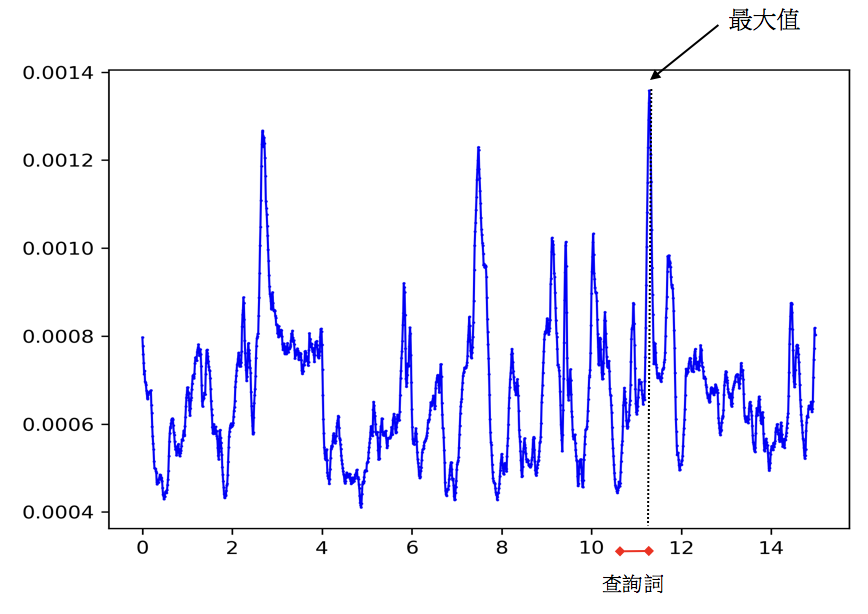
\includegraphics[scale=0.40]{images/ch4_softmax_att.png}\label{fig:att_softmax}}
\\
\subfloat[][平滑正規化]{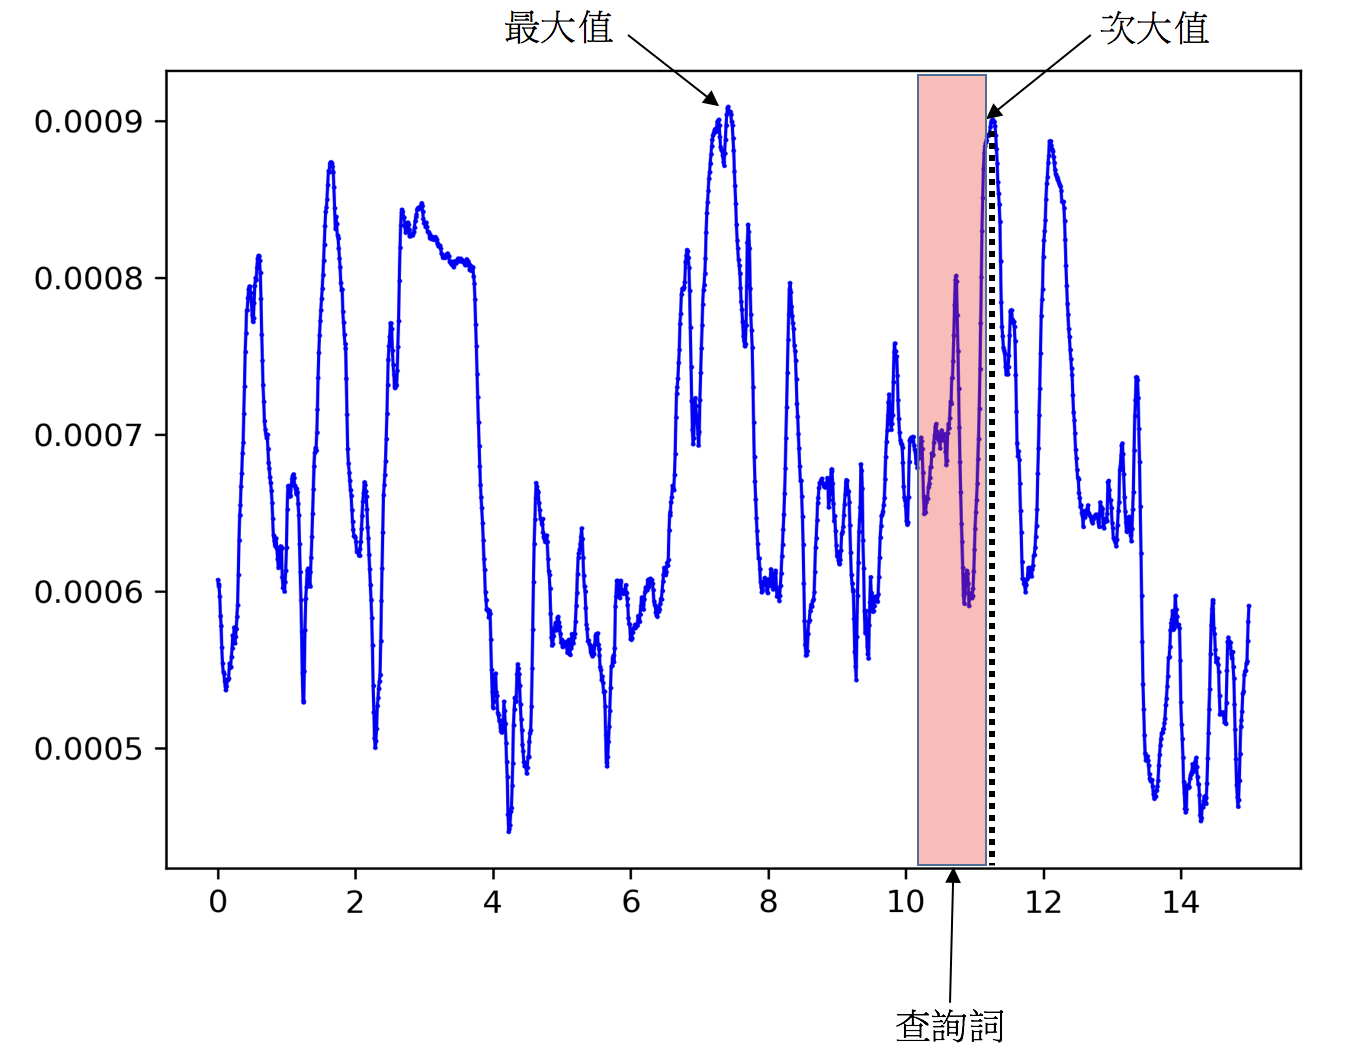
\includegraphics[scale=0.40]{images/ch4_sigmoid_att.png}\label{fig:att_sigmoid}}
\caption{專注式機制視覺圖}
\end{figure}
圖\ref{fig:att_softmax}跟圖\ref{fig:att_sigmoid}上的紅色區間為查詢詞在語音文件出現的部分,可以看出,兩者在查詢詞結束的位置專注式權重都非常的大,代表模型關注在長短期類神經網路看過整段查詢詞的輸出部分。然而兩者正規化機制仍有許多差異,平滑正規化的專注式權重值都較小,且關注的部分較多,使專制式權重最大值不是落在查詢詞結束處,而尖銳正規化的專注式權重較大,關注在少部分的地方,準確的關注在查詢詞結束處。兩種正規化機制各有利弊,取決於任務目的為何,若現在為語意理解,只關注某些部分,是無法了解整個語句意思,平滑正規化會有較好的效果。而現在的目標為口述詞彙偵測,只需要找出與查詢詞相關的部分,不需要關注太多較不相關的資訊,而使用尖銳正規化有較好的表現。
\begin{figure}[h]
\centering
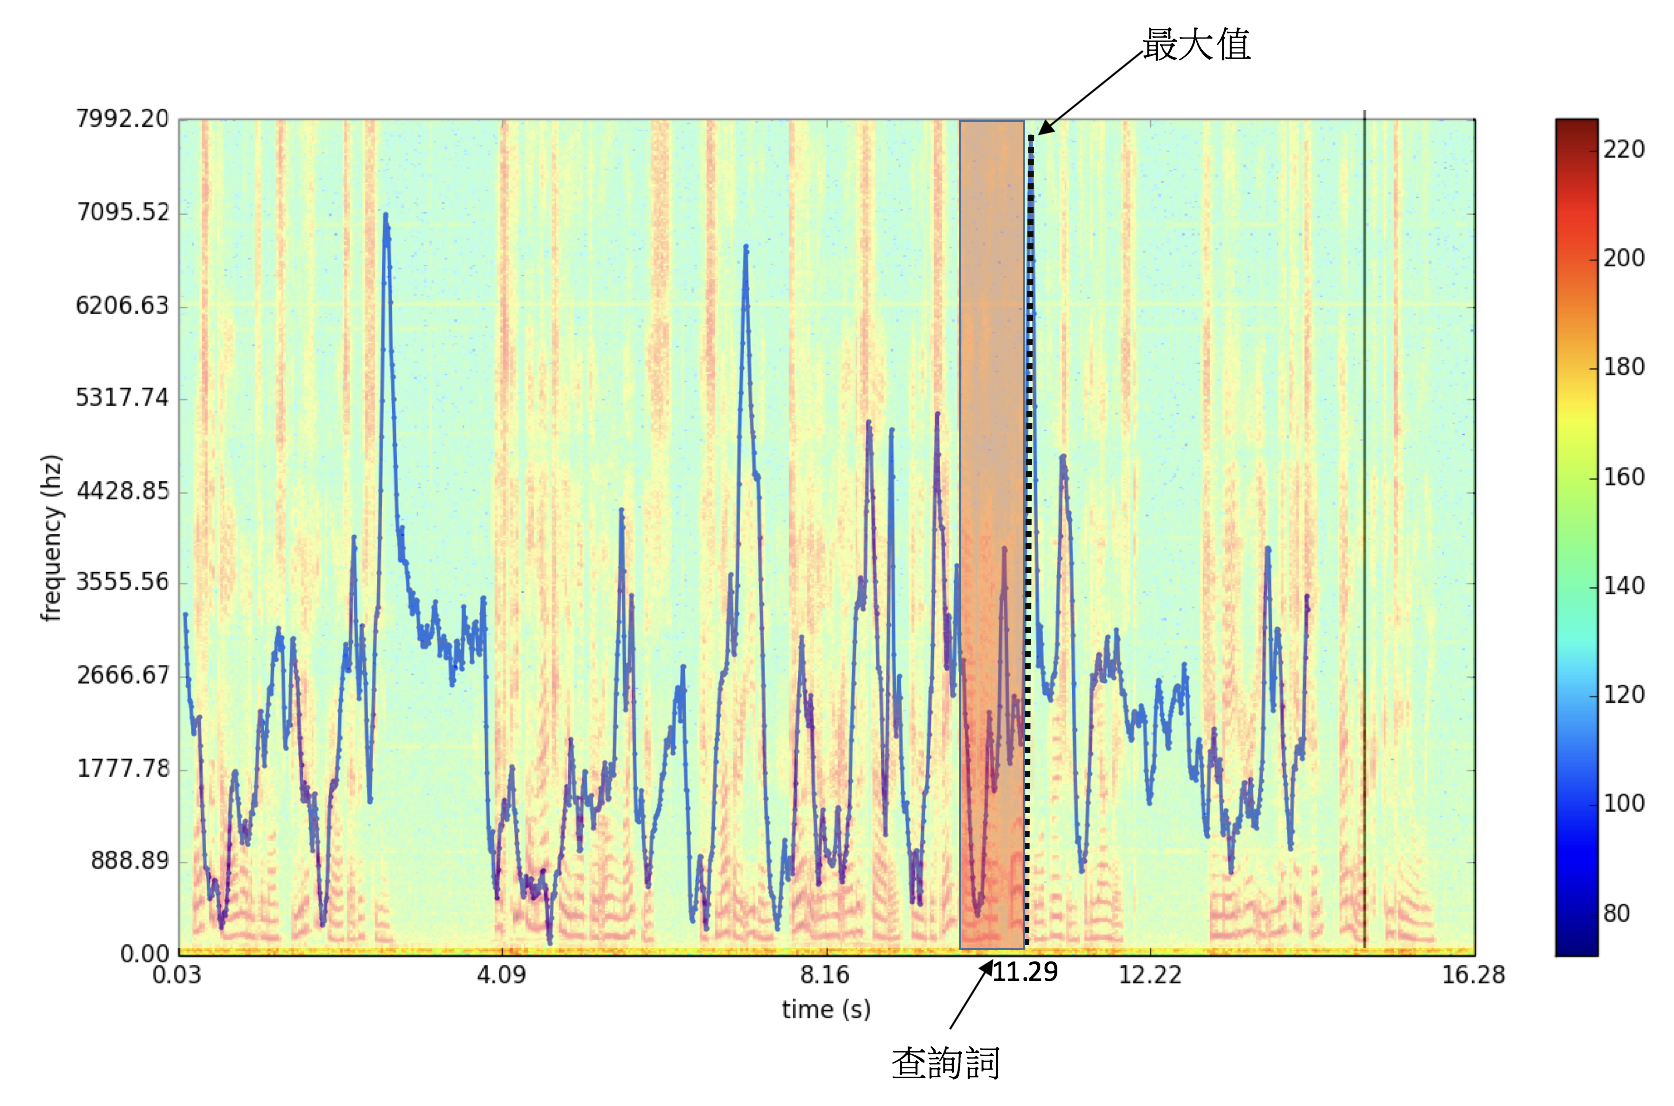
\includegraphics[scale=0.5]{images/ch4_softmax_spec.png} 
\caption{尖銳正規化頻譜圖}
\label{fig:spec_softmax}
\end{figure}

\begin{figure}[h]
\centering
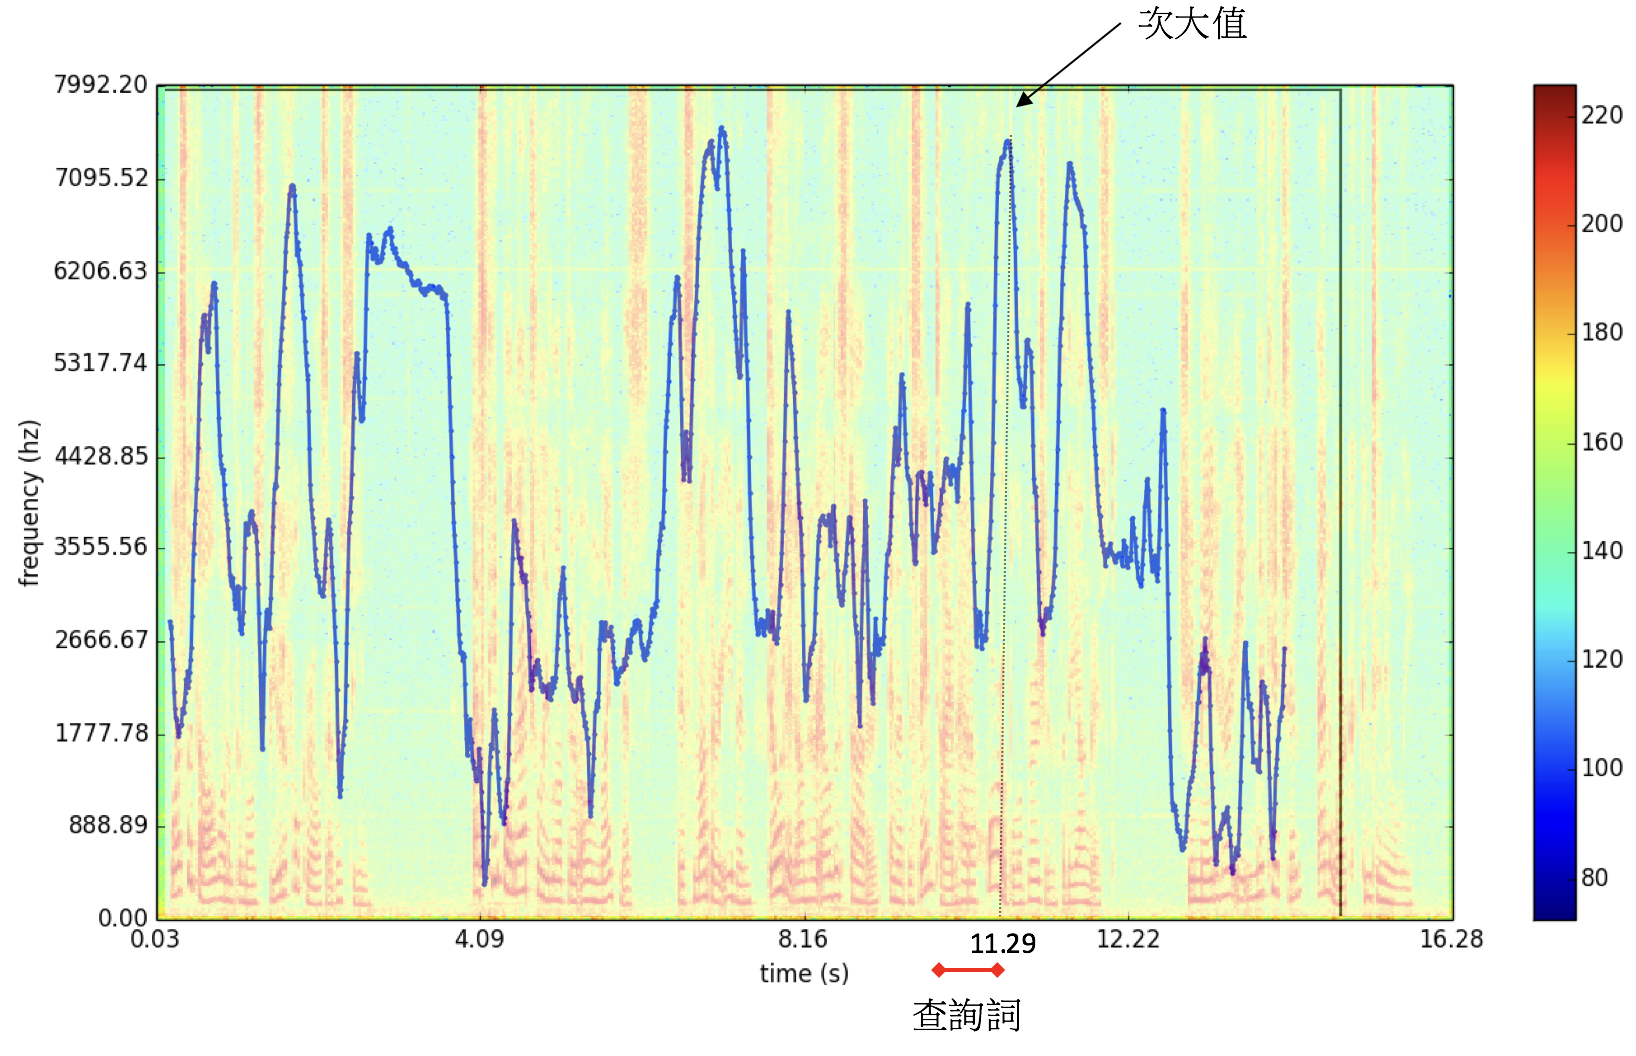
\includegraphics[scale=0.5]{images/ch4_sigmoid_spec.png} 
\caption{平滑正規化頻譜圖}
\label{fig:spec_sigmoid}
\end{figure}
圖\ref{fig:spec_softmax}跟圖\ref{fig:spec_sigmoid}為專注式機制作用在語音文件頻譜上的結果,可以看出模型並非隨機關注某些部分,而是幾乎關注一段語音的結束處。然而事前模型在資料中並無法得到每段語音文件的分段,而模型能夠直接就由資料從中學習出每段語音文件的分段並關注特別重要的部分,是蠻令人驚訝的,同時也證明了專注式機制能夠有效的取出重要的資訊,降低多餘的訊息的影響程度。
\end{itemize}
\subsection{非監督式訓練}

由於基準實驗為非監督式的方法,而專注式模型需要依賴標注好的資料才能夠進行訓練,用了許多訓練資料才贏過基準實驗。此節將直接利用動態時間規劃產生出查詢詞是否出現在文字中的答案,當成訓練資料給專注式模型訓練。而動態時間規劃的方法產生出的分數變化很大,所以將經過正規化調整使其落在$0$到$1$之間,對於類神經網路學習有很大幫助。對於每種查詢詞$j$中的各個分數$S_{ij}$會減去在查詢詞$j$中最小的分數在除上查詢詞中最大分數跟最小分數的差值,如式子\ref{norm}所示。

\begin{equation}
\label{norm}
\hat{S_{ij}} = \frac{(S_{ij}- \min_{k \in Q_j} S_{kj})} { (\max_{k \in
		Q_j} S_{kj} - \min_{k \in Q_j} S_{kj})}
\end{equation}
\begin{table}[ht]
	 \centering
	 \caption{非監督式學習}
	 \label{table:ch4_unsup}
	 \begin{tabular}{|c|c|c|c|c|}
		 \hline
		 \multicolumn{2}{|c|}{模型架構} & 測試集1 & 測試集2 & 測試集3 \\
		 \hline
		 \multicolumn{2}{|c|}{基準實驗} & 0.6173 & 0.5778 & 0.5678\\
		 \hline
		 \multicolumn{2}{|c|}{使用標註資料} &0.6523&0.6246 &0.5754 \\
		 \hline
		 \multicolumn{2}{|c|}{未使用標註資料} &0.6128&0.5893 &0.5548 \\
		 \hline
	   \end{tabular}
\end{table}

從表\ref{table:ch4_unsup}可以得出,專注式模型即便在非監督式學習的情況下也能夠跟基準模型表現抗衡。
\section{本章總結}
在本章中,我們引入了專注式機制,能夠使模型在產生語音文件向量表示時會因為查詢詞而關注在不同的部分,進而使語音文件向量表示變得更好。在實驗過程中,本章提出的模型能夠達到65.23\%的平均準確率,較基準實驗的61.3\%來得好。再者,語音查詢詞的語者改變,本章的模型仍能夠維持一定的水準,也證明了模型能夠學習到查詢詞的聲學模組,在實務應用上是可行的。同時,模型能夠藉由資料學習出文件聲音的段落,並且關注在查詢詞出現的部分。更進一步,將本章模型跟基準實驗的模型,相輔相成,平均準確率還能夠更上一層來到67.20\%。最後模型不使用標註的正確資料,而使用動態時間規劃的分數當作標注,仍能達到跟動態時間規劃一樣的表現,然而兩者的效率卻差了一截。
